\begin{Large}
	\vskip1cm
	\hskip0.5cm Software hierarchy:
	\begin{figure}[h]
		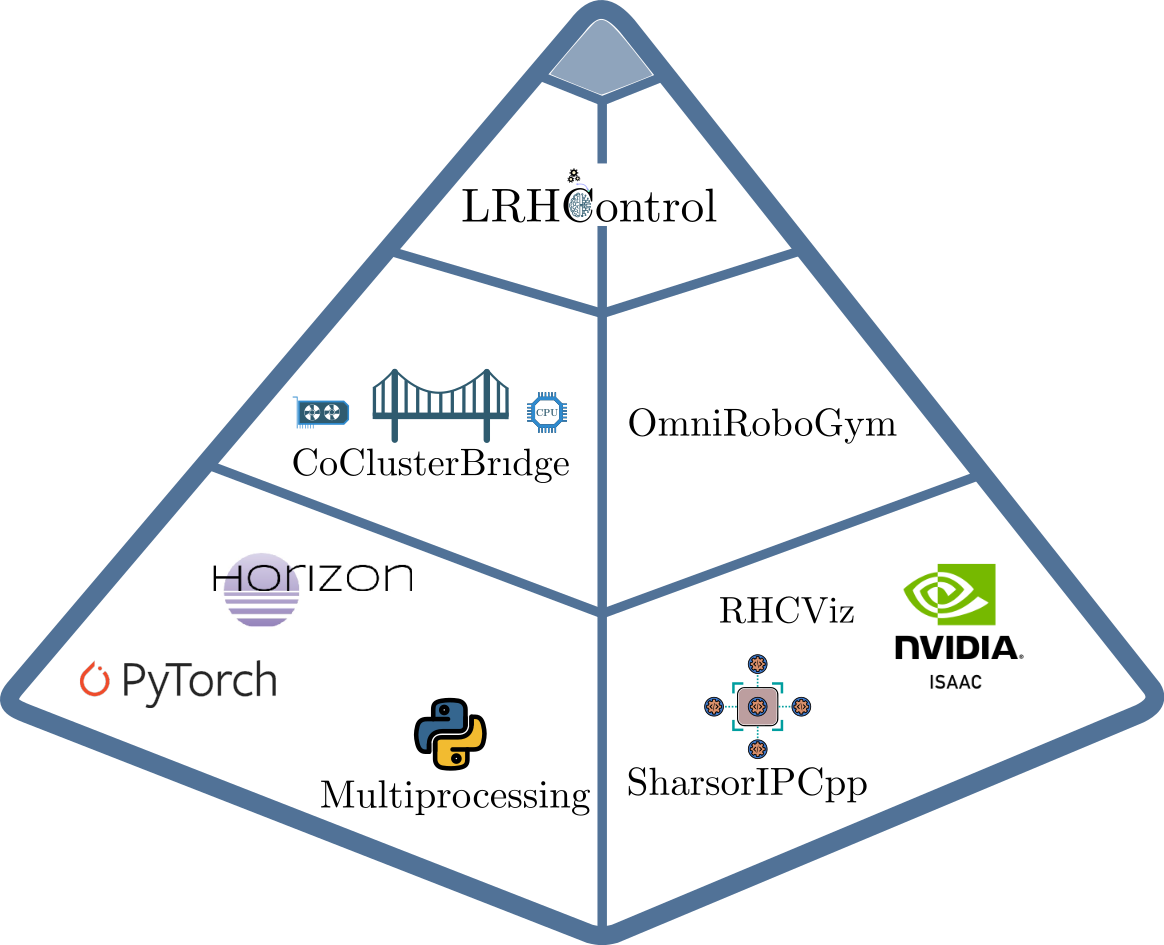
\includegraphics[width=0.6\textwidth]{docs/imgs/ecosystem.png}
	\end{figure}
	\begin{itemize}
		\item[$\rhd$] \textit{LRHControl} $\rightarrow$ main package; sim, train env, task implementations.\vskip0.3cm
		\item[$\rhd$] \textit{CoClusterBridge} $\rightarrow$ coordinates connection between simulator and cluster of RHCs\vskip0.3cm
		\item[$\rhd$] \textit{OmniRoboGym} $\rightarrow$ wrapper on top of IsaacSim; base sim env\vskip0.3cm
		\item[$\rhd$] \textit{SharsorIPCpp} $\rightarrow$ shared memory backend\vskip0.3cm
		\item[$\rhd$] Horizon (iLQR solver) $\rightarrow$ formulation of RHC controllers (CPU)\vskip0.3cm
		\item[$\rhd$] Multiprocessing $\rightarrow$ RHCs parallelization on CPU\vskip0.3cm
		\item[$\rhd$] GPU-accelerated simulation for data collection (IsaacSim)\vskip0.3cm
		\item[$\rhd$] PyTorch for DL components\vskip0.3cm
	\end{itemize}\vskip0.5cm
	\hskip0.5cm Architecture overview:
	\begin{figure}[h]
		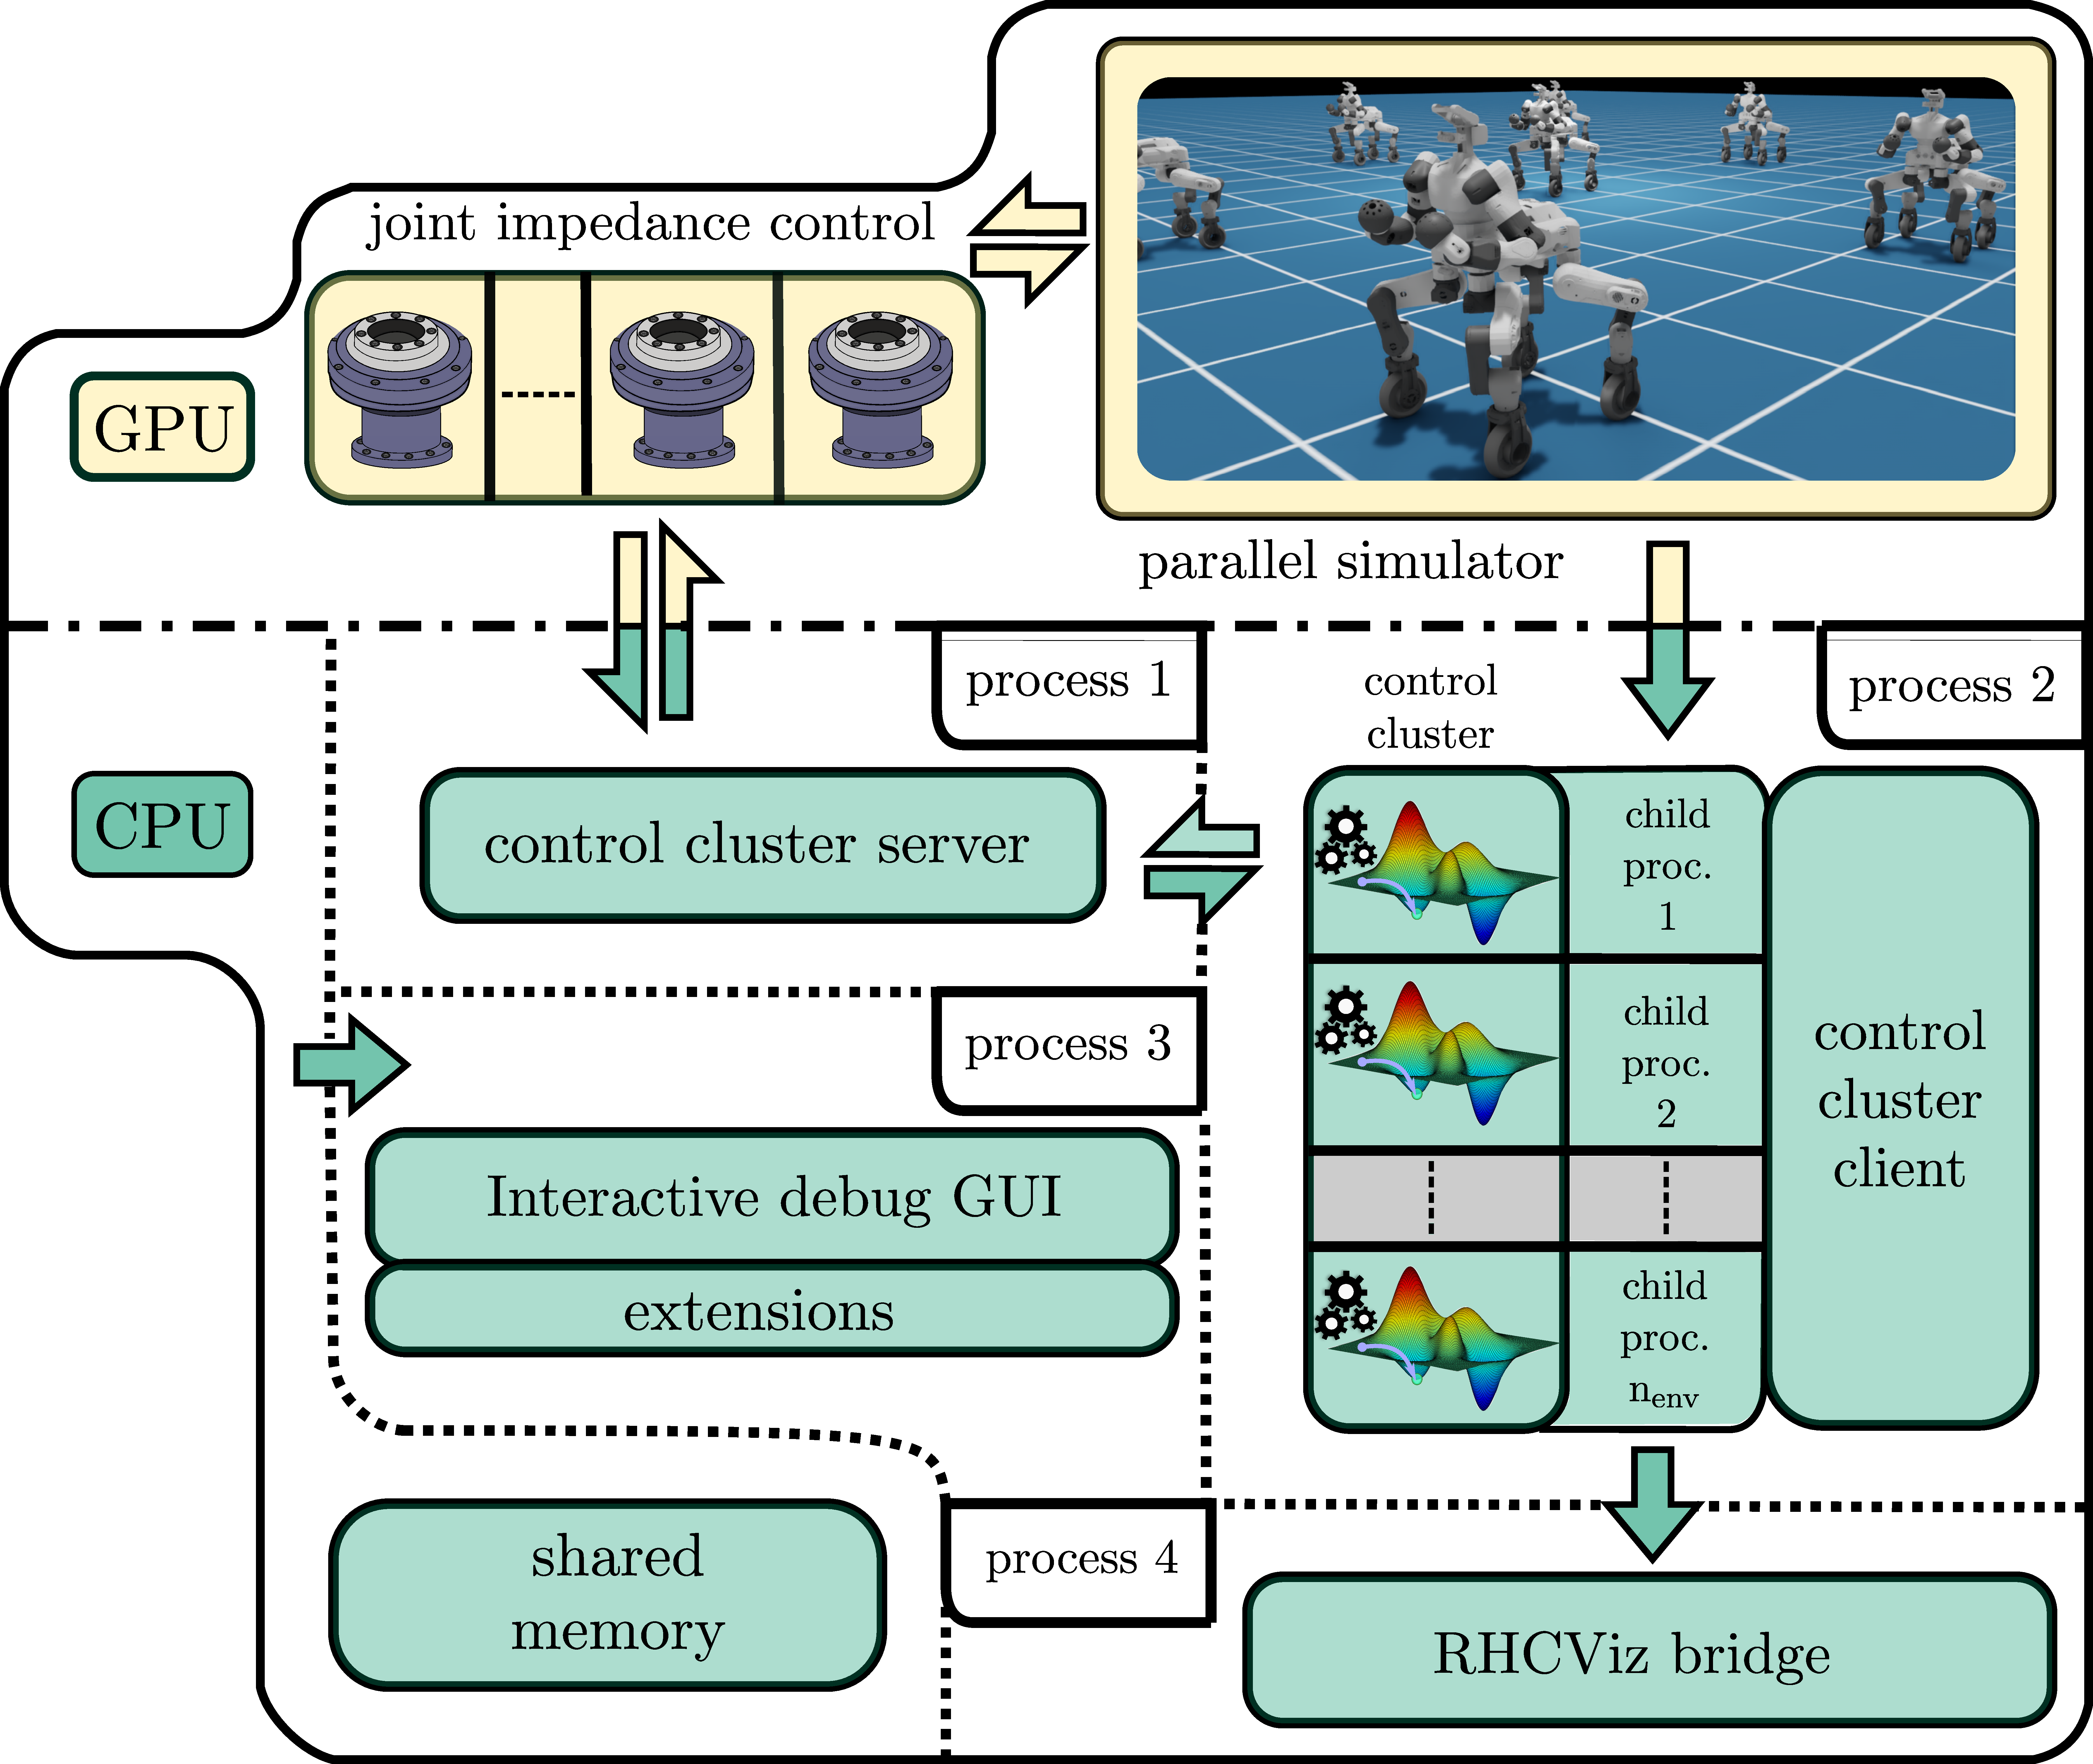
\includegraphics[width=0.7\textwidth]{docs/imgs/cocluster_arch_full.pdf}
	\end{figure}
	\vskip0.5cm
	\begin{itemize}
		\item[$\rhd$] Separate simulation and training env\vskip0.3cm
		\item[$\rhd$] RHCs run in parallel, synchronously w.r.t. simulator\vskip0.3cm
		\item[$\rhd$] Simulation stepping also parallel w.r.t. cluster solution\vskip0.3cm
		\item[$\rhd$] Extensible debugging GUI for monitoring RHCs, training and for easier RL task tuning\vskip0.3cm
		\item[$\rhd$] Single env visualization thanks to \textit{RHCViz}\vskip0.3cm
	\end{itemize}
	\vskip0.5cm
\end{Large}